\documentclass[12pt]{article}
\usepackage[english]{babel}
\usepackage[utf8]{inputenc}
\usepackage{amsmath, amssymb, amsthm}
\usepackage{graphicx}
\usepackage{hyperref}
\usepackage[margin=.75in]{geometry}
\usepackage{xcolor}
\usepackage{tikz}

\newcommand{\id}{\text{id}}
\newcommand{\od}{\text{od}}

\setlength{\topmargin}{0pt}
\setlength{\headsep}{0pt}
\textheight = 600pt

\title{Graph Theory \\ Homework 17}
\author{Ben Kallus and Josef Komissar}
\date{Due Monday, May 3}

\begin{document}
\maketitle

%% Be more precise with the word "cover"

\medskip\noindent\textbf{13.2}

    $G$:
    \begin{center} 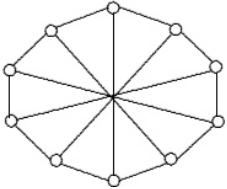
\includegraphics{1.png} \end{center}

\medskip\noindent\textbf{(a)}
    
    By Theorem 13.3, 3 = $\lceil \frac{10}{1 + 3} \rceil  \leq \gamma(G)$.
    The colored vertices in the following drawing of $G$ show a dominating set of size 3 for $G$:
    \begin{center} 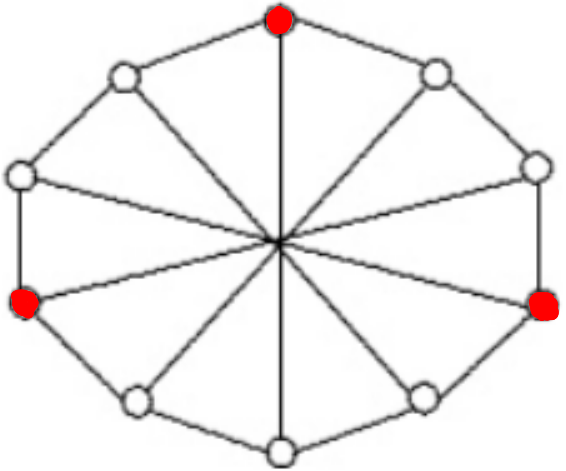
\includegraphics[scale=.4]{2.png} \end{center}
    Thus, $\gamma(G) = 3$.

\medskip\noindent\textbf{(b)}

    Note that $G$ is 3-regular, so each vertex in a set of vertices can contribute at most 3 to the number of vertices totally dominated by the set.
    Thus, $\gamma_t(G) \geq \lceil\frac{|V(G)|}{3}\rceil = \lceil\frac{10}3\rceil = 3$.
    The colored vertices in the following drawing of $G$ show a total dominating set of size 4 for $G$:
    \begin{center} 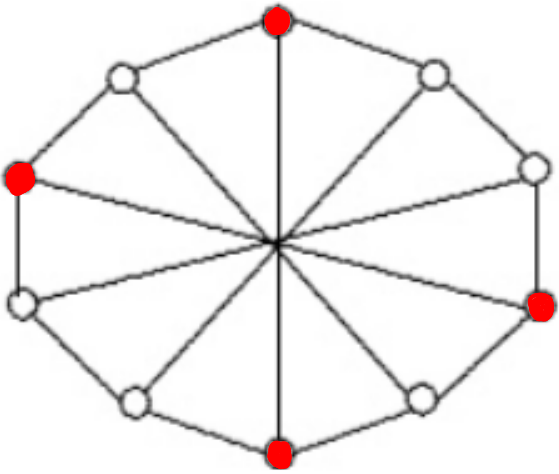
\includegraphics[scale=.4]{3.png} \end{center}
    Thus, $\gamma_t(G) = 4$.

\newpage\noindent\textbf{13.3}

\medskip\noindent\textbf{(2)}
    Note that a dominating set for $P_2$ can consist of a single vertex in $P_2$; either will do.
    Thus, $\gamma(P_2) = 1 = \lceil \frac 13 \rceil$.
    Let $n \geq 3$.
    By Theorem 13.3, $\lceil \frac n{3} \rceil = \lceil \frac n{1 + \Delta(P_n)} \rceil \leq \gamma(P_n)$.
    Label $P_n$'s vertices $v_0, \hdots, v_{n-1}$ such that $v_iv_{i+1} \in E(G)$ for all $0 \leq i \leq n - 2$.
    Suppose that 3 divides $n$.
    Then, $\{v_j \mid j \equiv 1 \mod 3 \text{ and } 0 \leq j \leq n - 1\}$ is a dominating set for $P_n$, because each vertex $v_j$ in the set covers $v_{j-1}, v_j, v_{j+1}$.
    Thus, if 3 divides $n$, $\gamma(P_n) \leq \frac n3 = \lceil \frac n3 \rceil$, so $\gamma(P_n) = \lceil \frac n3 \rceil$.
    Now, suppose that 3 does not divide $n$.
    Let $k$ be the remainder after dividing $n$ by 3.
    Note that because 3 does not divide $n$, $k \in \{1, 2\}$.
    Then, $\{v_j \mid j \equiv 1 \mod 3 \text{ and } 0 \leq j \leq n - 1\} \cup \{v_{n-1}\}$ is a dominating set of size $\lceil \frac n3 \rceil$, so $\gamma(P_n) = \lceil \frac n3 \rceil$.
    Thus, for all $n \geq 2$, $\gamma(P_n) = \lceil \frac n3 \rceil$.

    Observe that $\gamma_t(P_2) = 2$, because no total dominating set can be of cardinality 1.
    Let $n \geq 3$.
    Note that for any graph $G$, $\gamma_t(G + e) \leq \gamma_t(G)$ for all $e \in E(\overline G)$.
    Thus, $\gamma_t(C_n) \leq \gamma_t(P_n)$ for all $n \geq 3$.
    A total dominating set for $P_n$ can be constructed by first obtaining a total dominating set of size $\lceil \frac n2 \rceil$ for $C_n$, then removing some edge from $C_n$ with both endvertices not in the total dominating set.
    The existence of such an edge is clear from the proof from class of the total domination number for cycles.
    Thus, $\gamma_t(P_n) = \gamma_t(C_n) = \begin{cases} \lceil \frac n2 \rceil + 1 & n \equiv 2 \mod 4, \\ \lceil \frac n2 \rceil & \text{otherwise}. \end{cases}$

\newpage\noindent\textbf{(4)} 

    By Theorem 13.3, $\lceil \frac 8{1 + 3} \rceil = 2 \leq \gamma(Q_3)$.
    The following drawing shows a dominating set for $Q_3$ of size 2:
    \begin{center} 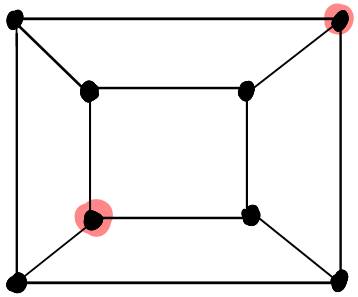
\includegraphics[scale=.5]{4.png} \end{center}
    Thus, $\gamma(Q_3) = 2$.

    All edges in $Q_3$ are symmetric, so we begin constructing a total dominating set for $Q_3$ by adding an arbitrary edge $vw$:
    \begin{center} 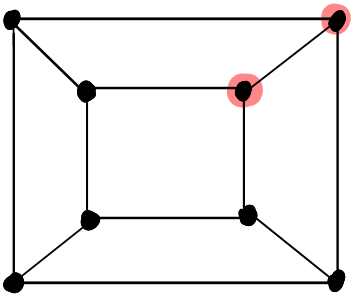
\includegraphics[scale=.5]{6.png} \end{center}
    There are two remaining vertices to be dominated, but neither is adjacent to $v$ or $w$, and they do not have a common neighbor that is adjacent to $v$ or $w$.
    Thus, there is no way to totally dominate them both with a single additional vertex.
    Thus, $\gamma_t(Q_3) \geq 4$.
    The following drawing shows a dominating set for $Q_3$ of size 4:
    \begin{center}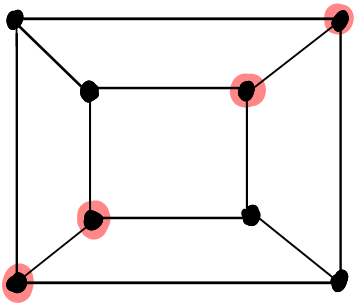
\includegraphics[scale=.5]{7.png}\end{center}
    Thus, $\gamma_t(Q_3) = 4$.
    
\newpage\noindent\textbf{(5)}

    By Theorem 13.3, $\lceil \frac 10{1+3} \rceil = 3 \leq \gamma(PG)$.
    The following drawing shows a dominating set for $PG$ of size $3$:
    \begin{center} 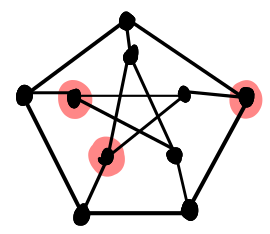
\includegraphics[scale=.7]{8.png} \end{center}
    Thus, $\gamma(PG) = 3$.

    By logic similar to Theorem 13.3, $\lceil \frac{10}{3} \rceil = 4 \leq \gamma_t(PG)$.
    This follows from the fact that each additional vertex added to the total dominating set can dominate at most $\Delta(PG) = 3$ other vertices.
    The following drawing shows a dominating set for $PG$ of size $4$:
    \begin{center} 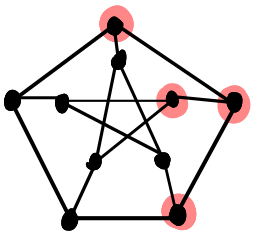
\includegraphics[scale=.7]{9.png} \end{center}
    Thus, $\gamma_t(PG) = 4$.

\newpage\noindent\textbf{13.8}

\medskip\noindent\textbf{(a)}

    The following drawing shows a minimal dominating set for $P_9$:
    \begin{center} 
\includegraphics[scale=.4]{10.png} \end{center}
    Note that this is a minimal dominating set because removing any vertex from the set leaves that vertex undominated.
    However, the vertices of $P_9$ that are not in this dominating set constitute a dominating set of size 4 for $P_9$.

\medskip\noindent\textbf{(b)}

    By \textbf{13.2(a)}, $\gamma(G) = 3$.
    Shown below is a minimal dominating set of size 5 for $G$:
    \begin{center} 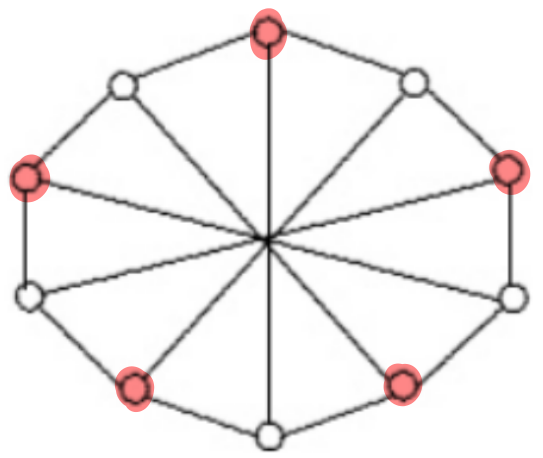
\includegraphics[scale=.4]{11.png} \end{center}
    This is a minimal dominating set because removing any vertex from the set leaves that vertex undominated.

\newpage\noindent\textbf{13.10} Proposition: There exists a graph $G$ and a minimal dominating set $S$ of $G$ such that $|S| - \gamma(G) \geq 2$.
\begin{proof}
    Consider the graph $G$ from \textbf{13.2(a)}.
    Then, by \textbf{13.8(b)}, there exists a minimal dominating set $S$ of size 5 for $G$.
    By \textbf{13.2(a)}, $\gamma(G) = 3$.
    Thus, $|S| - \gamma(G) = 2 \geq 2$.
\end{proof}

\newpage\noindent\textbf{13.12} Proposition: If $G$ is a graph with $\gamma(G) \geq 3$ and $\gamma(\overline G) \geq 3$, then the diameter of $G$ is 2.
\begin{proof}
    Let $G$ be a graph with $\gamma(G) \geq 3 and \gamma(\overline G) \geq 3$.
    Suppose that $G$ is disconnected.
    Consider two components of $G$, $U$ and $V$.
    Then, $\{u, v\}$ is a dominating set for $\overline G$ for all $u \in U, v \in V$.
    This follows from the fact that $u$ is adjacent in $\overline G$ to every vertex in every component of $G$ other than $U$, and $v$ is adjacent in $\overline G$ to every vertex in $U$.
    Then, $\gamma(\overline G) \geq 2$.
    This contradicts our assumption, so $G$ must be connected.

    Suppose that $\text{diam}(G) \geq 3$.
    Consider a pair of vertices $u,v$ in $G$ that are distance $\text{diam}(G)$ apart.
    Then, no neighbor of $u$ is adjacent to $v$ in $G$.
    Thus, for each neighbor $w$ of $v$ in $G$, $u$ is adjacent to $w$ in $\overline G$.
    Note that any vertex that is not a neighbor of $v$ in $G$ will be a neighbor of $v$ in $\overline G$, and any vertex that is not a neighbor of $u$ in $G$ will be a neighbor of $u$ in $\overline G$.
    Because $u$ is adjacent to $v$ in $\overline G$, we have shown that $\{u, v\}$ is a total dominating set for $\overline G$, which contradicts our assumption that $\gamma(\overline G) \geq 3$.

    Now, suppose that $\text{diam}(G) = 1$.
    Then, because $G$ is connected, it is a complete graph, so $\overline G$ is a null graph, and thus has no total dominating set.
    This contradicts our assumption that $\gamma(\overline G) \geq 3$.

    Thus, $\text{diam}(G) = 2$.

\end{proof}

\newpage\noindent\textbf{13.14}

For each $k \in \mathbb N$, a graph $G_k$ exists with the desired properties.
Let $k \in \mathbb N$.
We begin construction of $G_k$ with $P_k = (\{v_1, v_2, \hdots, v_k\}, \{v_1v_2, v_2v_3, \hdots, v_{k-1}v_k\})$.
Then, for each natural number $1 \leq i \leq k$, introduce two new vertices $u_i, w_i$ and add the edges $v_iu_i$ and $u_iw_i$.
\begin{center} 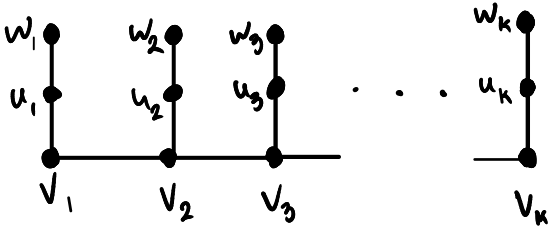
\includegraphics{12.png} \end{center}
Then, $\{u_i \mid 1 \leq i \leq k\}$ is a dominating set for $G_k$.
Thus, $\gamma(G_k) = k$, because a dominating set for $G_k$ must include at least one of $\{v_i, u_i, w_i\}$ for all $1 \leq i \leq k$.
Now, note that $\{v_i \mid 1 \leq i \leq k\} \cup \{u_i \mid 1 \leq i \leq k\}$ is a total dominating set for $G_k$.
Thus, $\gamma_t(G_k) \leq 2k$.
Suppose that there exists a total dominating set $S$ for $G_k$ that does not feature at least two of $\{v_i, u_i, w_i\}$ for all $1 \leq i \leq k$.
Let $j$ be a natural number between 1 and $k$ with the fewest of $w_j, u_j, v_j$ present in $S$.
Then, if none of these vertices are present in $S$, $w_j$ would not be totally dominated by $S$.
Thus, at least one of these vertices must be in $S$.
If only $u_j$ is present in $S$, then $u_j$ is not totally dominated by $S$.
If only $w_j$ is present in $S$, then $w_j$ is not totally dominated by $S$.
If only $v_j$ is present in $S$, then $w_j$ is not totally dominated by $S$.
Thus, it must be that any dominating set for $G_k$ contains at least two of $\{v_i, u_i, w_i\}$ for all $1 \leq i \leq k$.
Thus, $\gamma_t(G_k) \geq 2k$.
Thus, $\gamma_t(G_k) = 2k$,.
Thus, $G_k$ satisfies the constraints given.

\end{document}
